\documentclass[12pt]{article}

\usepackage{times}
\usepackage{textcomp}
\usepackage{listings}
\usepackage{fullpage}
\usepackage{color}
\usepackage{hyperref} 
\usepackage{pst-tree} 
\usepackage{verbatim} 
\usepackage{graphicx}
\usepackage{amsmath,amsfonts,amssymb,amsthm}
\graphicspath{{./}}
\usepackage{courier}

\lstset{language=C, keywordstyle={\bfseries \color{red}}, basicstyle=\footnotesize\ttfamily}

\author{Clement Tsang}

\begin{document}

\begin{center}
\Large\textbf{CS 241, Lecture 20: Code Generation for Procedures}
\end{center}

\section{Procedures}
\begin{itemize}
    \subsection{Differences between generic procedures and wain:}
        \item We don't need imports
        \item Need to update \lstinline[mathescape]{$\$$29}
        \item Save registers
        \item Restore registers and stack and \lstinline[mathescape]{jr $\$$31} at the end
    \subsection{Saving and Restoring Registers, Arguments}
        \item Our convention is that the caller saves \lstinline[mathescape]{$\$$31}, and the callee will save registers that it will modify and restore in the end.
        \item The caller also saves register \lstinline[mathescape]{$\$$29},  
        \item We now need to store the arguments to pass to a function.
        \item We can't store this on registers, we need to store this on the stack.
        \item We get the following code for a \lstinline[mathescape]{factor $\rightarrow$ ID(expr1, \dots , exprn)}:
\begin{lstlisting}[mathescape, numbers=none, breaklines=true]
code(factor) = push(s29) 
               + push(s31)
               + code(expr1) 
               + push(s3)
               + code(expr2) 
               + push(s3)
               + $\dots$
               + code(exprn)
               + push(s3)
               + lis s5
               + .word ID
               + jalr s5
               + pop n times
               + pop(s31) 
               + pop(s29)
\end{lstlisting}
        \item For \lstinline[mathescape]{procedures $\rightarrow$ int ID(params) dcls statements RETURN expr;}, we have:
\begin{lstlisting}[mathescape, numbers=none, breaklines=true]
code(procedure) = sub s29, s30, s4
                  ;save registers we are going to use:
                  + push regs
                  + code(dcls) ;local vars
                  + code(stmts)
                  + code(expr)
                  + pop regs ;restore saved regs
                  + add s30, s29, s4
                  + jr s31
\end{lstlisting}
        $\dots$except nope, this isn't going to be that easy!  We have some problems!
    \subsection{Stack}
        \item Basically, the issue with our previous approach is that our parameter offsets will be below register \$29$\dots$ which isn't good!  This also causes problems with local variables since the saved registers come before local variables.
        \item Essentially, the issue is that our saved registers of our function would come before our local vars$\dots$ like so:\\
            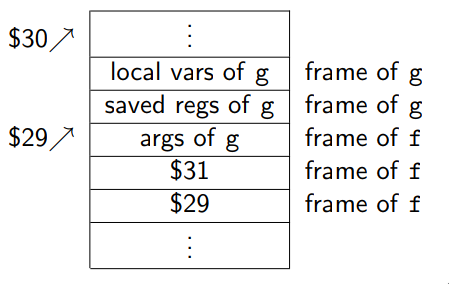
\includegraphics[scale=0.5]{stack_1.png}
        \item We rewrite our procedure code:
\begin{lstlisting}[mathescape, numbers=none, breaklines=true]
code(procedure) = sub s29, s30, s4
                  + push dcls ;local vars
                  + push regs ;save used regs
                  + code(stmts)
                  + code(expr)
                  + pop regs ;restore saved regs
                  + add s30, s29, s4
                  + jr s31
\end{lstlisting}
        where \lstinline[mathescape]{push dcls} means to run \lstinline[mathescape]{code(dcls)} and push them all to the stack.
        \item Now our stack looks like this:\\
            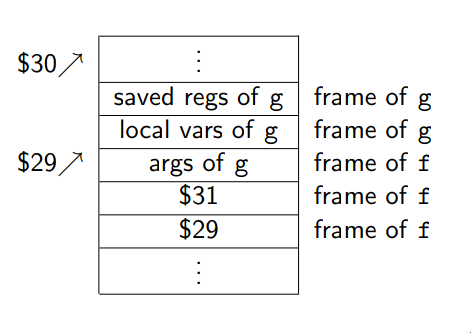
\includegraphics[scale=0.5]{stack_2.png}
        \item In summary:
            \begin{itemize}
                \item Parameters should have positive offsets
                \item Local variables should have non-positive offsets
                \item Symbol tables should have added 4 $\times$ \#params to each entry in the table
            \end{itemize}
    \subsection{Labels}
        \item What if we have a function called \lstinline[mathescape]{print} in our WLP4 code?  We would have duplicate labels with our reserved label for printing!
        \item This is also a problem with \lstinline[mathescape]{new, init, delete}.  We could just ban these keywords$\dots$ but that seems a bit much.
        \item Luckily there's an easy and simple solultion --- just append an \lstinline[mathescape]{F} in front of our labels for functions!  So our code for factors into function calls  would now be:
\begin{lstlisting}[mathescape, numbers=none, breaklines=true]
code(factor) = push(s29) 
               + push(s31)
               + code(expr1) 
               + push(s3)
               + code(expr2) 
               + push(s3)
               + $\dots$
               + code(exprn)
               + push(s3)
               + lis s5
               + .word FID ;append F in front of the ID
               + jalr s5
               + pop n times
               + pop(s31) 
               + pop(s29)
\end{lstlisting}
    \subsection{Optimization}
        \item \textbf{Constant folding:} if we are constantly using the same constant repeatedly, we can just load it \emph{once} instead of multiple times!
        \item If you aren't going to ever use a local variable, you could remove the stack entry part, saving more space.
        \item \textbf{Common subexpression elimination:} If you see the same value being computed twice, you can instead compute that value ONCE and call it on itself.  For example, $(a - b) * (a-b)$ can be resolved by solving $(a-b)$ once then calling \lstinline[mathescape]{mult} on itself.
        \item \textbf{Dead code elimination:} Remove code that will never execute!  
        \item \textbf{Register allocation:}
            \begin{itemize}
                \item Accessing variables on RAM is expensive$\dots$ and we have unused registers \$14 to \$28... so let's use them!
                \item But \emph{what} should we store here?  Most used?  Recently used?
                \item We try to do it such that variables are in registers when in a live range, and remove them when outside of this range.
                \item For example, given this code:
\begin{lstlisting}[mathescape, numbers=none, breaklines=true]
int wain(int a, int b) {
    int x = 0; int y = 0; int z = 0;
    x = 3;
    y = 10;
    println(x);
    z = 7;
    y = y - x;
    y = y - z;
    println(z);
    return z;
}
\end{lstlisting}
                the live ranges are \lstinline[mathescape]{x}: lines 3 to 7, \lstinline[mathescape]{y}: lines 4-8, and \lstinline[mathescape]{z}: lines 6 to 10.
            \item Note that in this example, we could easily just stick all three variables into registers.
            \end{itemize}
        \item \textbf{Strength reduction:} Use addition instead of multiplication if possible.
        \item \textbf{Inlining procedures:} Consider the following:
\begin{lstlisting}[mathescape, numbers=none, breaklines=true]
int f (int a, int b) {
    return a + b;
}

int wain(int a, int b) {
    return f(a, b);
}
\end{lstlisting}
        This is equal to:
\begin{lstlisting}[mathescape, numbers=none, breaklines=true]
int wain(int a, int b) {
    return a + b;
}
\end{lstlisting}
        This eliminates the overhead of a function call.  Note this isn't \emph{always} shorter, but it is if \lstinline[mathescape]{f}'s body is shorter than the code to call it, and/or if we are calling it only a few times.
        \item \textbf{Tail recursion:} 
            \begin{itemize}
                \item Given code where the last operation in a function is returning a value when recursing, we can reuse the current stack frame to save operations$\dots$ but we can't do this in WLP4 as we don't allow for return statements in if statements!
                \item But if we could$\dots$ then all we need to do is in our \lstinline[mathescape]{factor} code, reset stack pointer and \lstinline[mathescape]{jr} to the function label versus popping args, saving \$31 or \$29.
            \end{itemize}
        \item Okay but$\dots$ how do we do these optimizations?  What we often do is first, rewrite our code \emph{in our current language} - this is called \textbf{intermediate code}.  So in our case, rewrite our stuff to work better \emph{in} WLP4, THEN we run this through our compiler!
\end{itemize}

\end{document}

